\documentclass[12pt, a4paper]{article}
\usepackage{enumitem}
\usepackage{float}
\usepackage[left=2cm, right=2cm, top=2cm, bottom=2cm]{geometry}
\usepackage{graphicx}
\usepackage[colorlinks, urlcolor=blue]{hyperref}
\usepackage{minted}
\usepackage{xeCJK}

\renewcommand\arraystretch{1.5}
\setCJKmainfont[AutoFakeBold=1.5]{新細明體}
\setlength{\parindent}{0pt}

\setminted{
  frame=single,
  tabsize=2,
}

\title{
  \vspace{-1cm}
  Network Administration/System Administration\\
  (NTU CSIE, Spring 2024)\\
  Homework \#11 - Nginx
}
\author{\Large B12902110 呂承諺}

\begin{document}
  \maketitle

  \section*{Web Terminology}
  \begin{enumerate}
    \item \phantom{}\vspace{-\baselineskip}

    \begin{tabular}{|c|c|c|}
      \hline
      & \textbf{Apache} & \textbf{Nginx} \\\hline
      Asynchronous, event-driven & Via event MPM & Native \\\hline
      Mail proxy support & No & Yes \\\hline
      License & Apache License 2.0 & 2-Clause BSD License \\\hline
    \end{tabular}
    \vspace{\baselineskip}

    \textbf{References}
    \begin{itemize}
      \item \href{https://en.wikipedia.org/wiki/Apache_HTTP_Server}{Apache HTTP Server - Wikipedia}
      \item \href{https://en.wikipedia.org/wiki/Nginx}{Nginx - Wikipedia}
      \item \href{https://www.nginx.com/blog/thread-pools-boost-performance-9x/}{Boosting NGINX Performance 9x with Thread Pools}
      \item \href{https://httpd.apache.org/docs/2.4/mod/event.html}{event - Apache HTTP Server Version 2.4}
      \item \href{https://www.digitalocean.com/community/tutorials/apache-vs-nginx-practical-considerations}{Apache vs Nginx: Practical Considerations  | DigitalOcean}
    \end{itemize}

    \item A \textbf{static web server} sends out files hosted on the server as-is.

    A \textbf{dynamic web server} constructs the response content during runtime with
    resources such as HTML templates, databases, or API calls.

    A static web server usually handle requests faster than a dynamic web server
    because no content has to be built by the server.

    \textbf{References}
    \begin{itemize}
      \item \href{https://developer.mozilla.org/en-US/docs/Learn/Common_questions/Web_mechanics/What_is_a_web_server}{What is a web server? - Learn web development | MDN}
      \item \href{https://en.wikipedia.org/wiki/Dynamic_web_page}{Dynamic web page - Wikipedia}
    \end{itemize}

    \pagebreak
    \item \textbf{Client-side rendering (CSR)}: The server sends a minimal HTML page
    to the client, and the client then renders the main content dynamically using
    JavaScript, which may include additional HTTP fetches and API calls.
    A benefit of CSR is a smooth and interactive user experience, just like
    using an app.

    \textbf{Server-side rendering (SSR)}: When the client requests a page, the server
    renders the complete page with data from databases or API calls, and then sends the
    response to the client. A benefit of SSR is better search engine optimization than CSR.

    \textbf{Static-site generation (SSG)}: The whole website is rendered into
    static pages during build time. The main benefit of SSG excellent performance and
    fast loading times.

    \textbf{Incremental static regeneration (ISR)}: ISR allows static pages
    to be built on a per-page basis. A page will be generated upon first request,
    and future requests within a certain amount of time will be served from cache.
    It offers better performance than SSR because only certain pages rather than
    the whole website has to be regenerated upon content change.

    \textbf{References}
    \begin{itemize}
      \item \href{https://www.shubo.io/rendering-patterns/}{[教學] SSR 與 CSR 深度解析:從渲染方式到效能優化 - Shubo 的程式開發筆記}
      \item \href{https://bootcamp.uxdesign.cc/understanding-csr-ssr-ssg-and-isr-a-next-js-perspective-fcaf36686de6}{Understanding CSR, SSR, SSG, and ISR: A Next.js Perspective | by Aditya Kumar Tiwari | Bootcamp}
      \item \href{https://www.educative.io/answers/ssr-vs-csr-vs-isr-vs-ssg}{SSR vs CSR vs ISR vs SSG}
      \item \href{https://nextjs.org/docs/pages/building-your-application/data-fetching/incremental-static-regeneration}{Data Fetching: Incremental Static Regeneration (ISR) | Next.js}
    \end{itemize}

    \item A \textbf{proxy} is an intermediate between the client and server. When the client
    wants to access a resource, the request goes to the proxy instead of directly to
    the server. The proxy performs the request to the server, receives the response,
    and then sends the response back to the client.

    Some benefits of a proxy are:
    \begin{itemize}
      \item \textbf{Security}: Mask the IP address of the client.
      \item \textbf{Filtering}: Filter out unwanted content.
      \item \textbf{Caching}: Cache frequently accessed resources for performance.
    \end{itemize}

    \textbf{References}
    \begin{itemize}
      \item \href{https://en.wikipedia.org/wiki/Proxy_server}{Proxy server - Wikipedia}
    \end{itemize}

    \item A \textbf{reverse proxy} is a proxy server that acts to clients just like a
    normal web server, but actually forwards requests to and responses from one or more web
    servers behind it.

    Some benefits of a reverse proxy server are:
    \begin{itemize}
      \item \textbf{Load balancing}: Distribute load among multiple servers.
      \item \textbf{Security}: Only the reverse proxies have to be exposed to the public,
      while the actual web servers can be hidden behind a firewall.
      \item \textbf{Caching}: Cache frequently accessed resources for performance.
    \end{itemize}

    \textbf{References}
    \begin{itemize}
      \item \href{https://en.wikipedia.org/wiki/Reverse_proxy}{Reverse proxy - Wikipedia}
    \end{itemize}
  \end{enumerate}

  \pagebreak
  \section*{Web Server Configurations}
  \begin{enumerate}[resume]
    \item \textbf{Steps}
    \begin{enumerate}[label=(\arabic*)]
      \item Run the following commands to prepare the VM.
      \begin{Verbatim}[frame=single]
$ cp -r /tmp2/nasa-hw11 /tmp2/b1290110
$ cd /tmp2/b12902110/nasa-hw11
$ qemu-img create -f qcow2 disk0.qcow2 20G
      \end{Verbatim}
      \item Create \verb|/tmp2/b12902110/nasa-hw11/run_vm.sh| as the following.
      \inputminted[fontsize=\scriptsize]{shell}{run_vm.sh}
      \item Boot up the VM, connect to it via QEMU's VNC, and follow the Debian installation guide. After the installation finished, reboot into the VM.
      \item Configure sudo as the root user.
      \begin{Verbatim}[frame=single]
$ su -
# apt install -y sudo
# usermod -aG sudo b12902110
      \end{Verbatim}
      \item Re-login as user b12902110. Install the necessary package for our
      web server.
      \begin{Verbatim}[frame=single]
$ sudo apt install -y nginx
      \end{Verbatim}
      \item Start the nginx service.
      \begin{Verbatim}[frame=single]
$ sudo systemctl start nginx.service
      \end{Verbatim}
    \end{enumerate}

    \textbf{Result}

    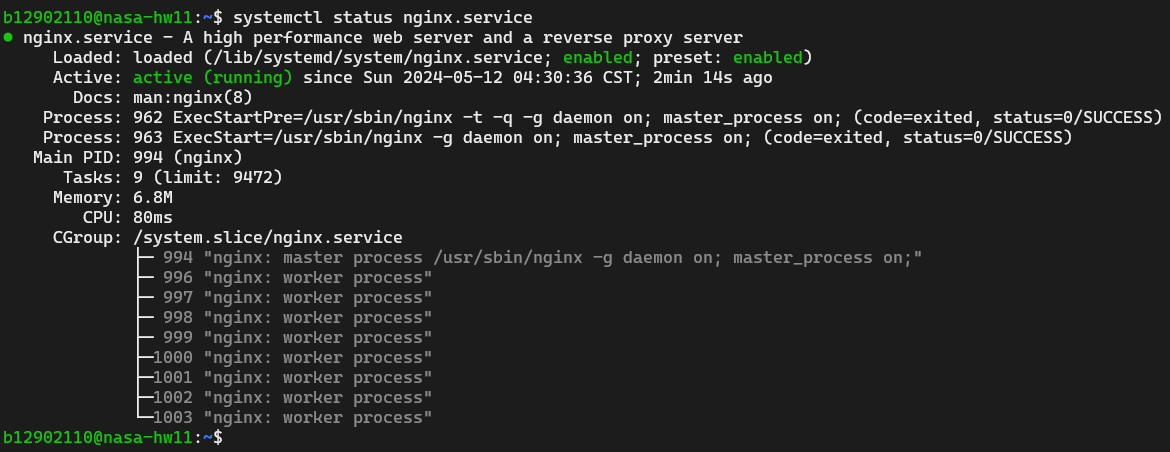
\includegraphics[width=0.9\textwidth]{6_result.png}

    \textbf{References}
    \begin{itemize}
      \item \href{https://www.linuxquestions.org/questions/linux-newbie-8/command-usermod-not-found-385901/}{command usermod not found}
    \end{itemize}

    \item \textbf{Steps}
    \begin{enumerate}[label=(\arabic*)]
      \item Install \verb|ufw|.
      \begin{Verbatim}[frame=single]
$ sudo apt install -y ufw
      \end{Verbatim}
      \item Configure firewall rules with the following commands.
      \begin{Verbatim}[frame=single]
$ sudo ufw default deny
$ sudo ufw allow 22
$ sudo ufw allow 80
$ sudo ufw allow 443
$ sudo ufw enable
      \end{Verbatim}
    \end{enumerate}

    \textbf{Result}

    This part is done after the last problem, so we have more services than an HTTP
    and an SSH service.

    In the QEMU console, add another port forwarding rule: 11088 on the host to
    8888 on the VM.
    \begin{Verbatim}[frame=single]
(qemu) hostfwd_add tcp::11088-:8888
    \end{Verbatim}

    Therefore, we have 4 port forwarding rules.

    \begin{tabular}{|ll|}
      \hline
      \textbf{Source} & \textbf{Destination} \\\hline
      ws2.csie.ntu.edu.tw:11022 & nasa-hw11:22 \\
      ws2.csie.ntu.edu.tw:11080 & nasa-hw11:80 \\
      ws2.csie.ntu.edu.tw:11043 & nasa-hw11:443 \\
      ws2.csie.ntu.edu.tw:11088 & nasa-hw11:8888 \\
      \hline
    \end{tabular}

    All of the 4 ports has a service running on it.

    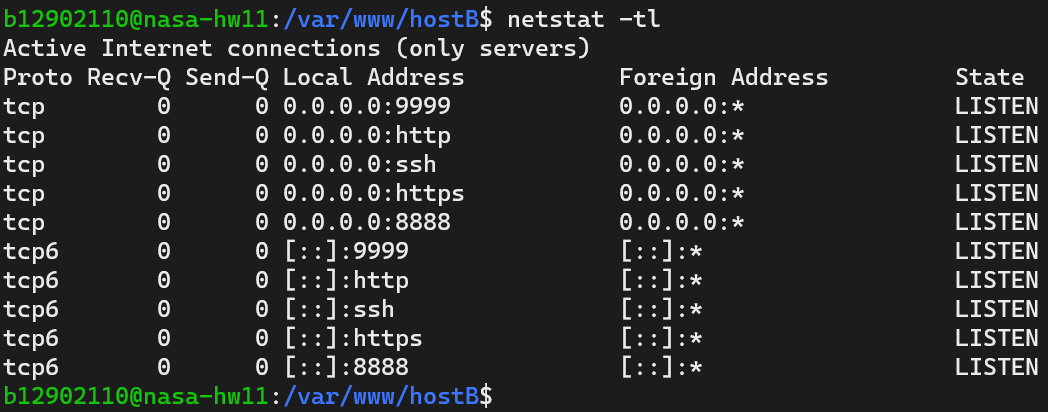
\includegraphics[width=0.8\textwidth]{7_netstat.png}

    \pagebreak
    However, only ports 22, 80, and 443 are accessible from outside
    the VM.

    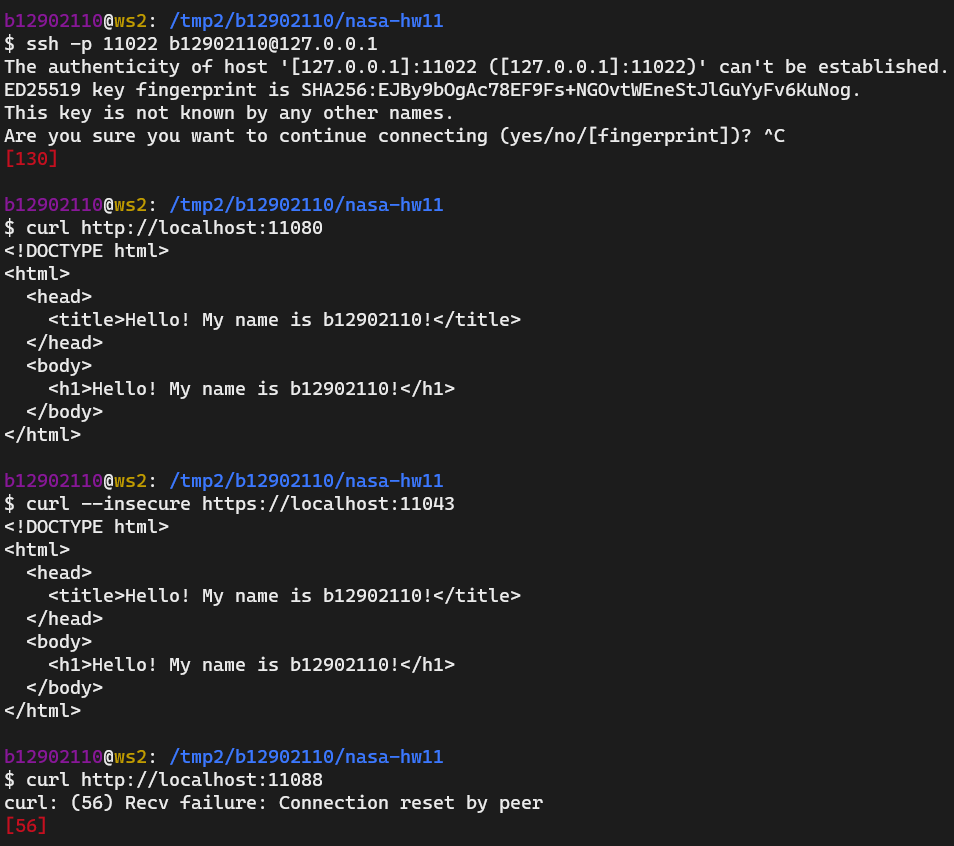
\includegraphics[width=0.8\textwidth]{7_access.png}

    \vspace{\baselineskip}
    \textbf{References}
    \begin{itemize}
     \item \href{https://www.digitalocean.com/community/tutorials/opening-a-port-on-linux}{How To Open a Port on Linux  | DigitalOcean}
     \item \href{https://www.digitalocean.com/community/tutorials/how-to-set-up-a-firewall-with-ufw-on-ubuntu}{How to Set Up a Firewall with UFW on Ubuntu  | DigitalOcean}
    \end{itemize}

    \pagebreak
    \item \textbf{Steps}

    Create \verb|/var/www/html/index.html| as the following.
    \inputminted{html}{server/var/www/html/index.html}

    \textbf{Result}

    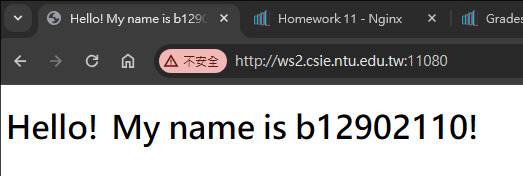
\includegraphics[width=0.6\textwidth]{8_result.png}

    \pagebreak
    \item \textbf{Steps}
    \begin{enumerate}[label=(\arabic*)]
      \item Add the following \verb|location| block into
      \verb|/etc/nginx/sites-available/default|.
      \begin{Verbatim}[frame=single]
server {
  ...

  location ~ ^/~(.*?)/(.*) {
    alias /home/$1/htdocs/$2;
  }

  ...
}
      \end{Verbatim}
      \item Run the following commands.
      \begin{Verbatim}[frame=single]
$ chmod 755 /home/b12902110
$ mkdir /home/b12902110/htdocs
      \end{Verbatim}
      \item Create \verb|/home/b12902110/htdocs/index.html| as the following.
      \inputminted{html}{server/home/b12902110/htdocs/index.html}
      \item Reload the nginx service.
      \begin{Verbatim}[frame=single]
$ sudo systemctl reload nginx.service
      \end{Verbatim}
    \end{enumerate}

    \textbf{Result}

    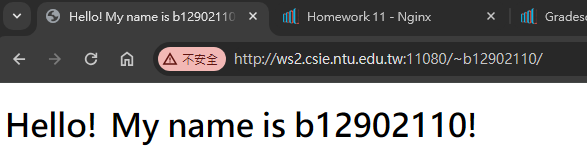
\includegraphics[width=0.6\textwidth]{9_result.png}

    \vspace{\baselineskip}
    \textbf{References}
    \begin{itemize}
      \item \href{https://stackoverflow.com/questions/42605637/nginx-user-public-home-without}{nginx user public home without ~ - Stack Overflow}
      \item \href{https://nginx.org/en/docs/beginners_guide.html}{Beginner's Guide}
      \item \href{https://nginx.org/en/docs/http/ngx_http_core_module.html}{Module ngx\_http\_core\_module}
    \end{itemize}

    \pagebreak
    \item \textbf{Steps}
    \begin{enumerate}[label=(\arabic*)]
      \item Add the following \verb|location| block into
      \verb|/etc/nginx/sites-available/default|.
      \begin{Verbatim}[frame=single]
server {
  ...

  location = /secret.html {
    allow 192.168.28.0/24;
    deny all;
  }

  ...
}
      \end{Verbatim}

      \item Reload the nginx service.
      \begin{Verbatim}[frame=single]
$ sudo systemctl reload nginx.service
      \end{Verbatim}
    \end{enumerate}

    \textbf{Result}

    Before restriction:

    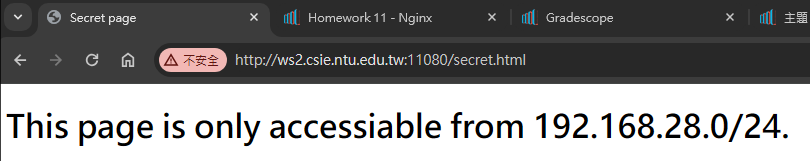
\includegraphics[width=0.6\textwidth]{10_result_before.png}

    After restriction:

    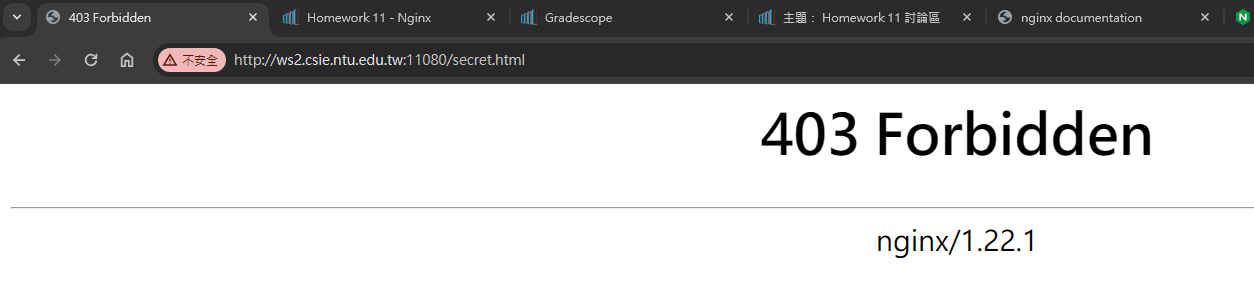
\includegraphics[width=0.8\textwidth]{10_result_after.png}

    \vspace{\baselineskip}
    \textbf{References}
    \begin{itemize}
      \item \href{https://nginx.org/en/docs/http/ngx_http_access_module.html}{Module ngx\_http\_access\_module}
    \end{itemize}

    \pagebreak
    \item \textbf{Steps}

    View the last few lines of \verb|/var/log/nginx/access.log|/
    \begin{Verbatim}[frame=single]
$ sudo tail /var/log/nginx/access.log
    \end{Verbatim}

    \textbf{Result}

    Chrome DevTools:

    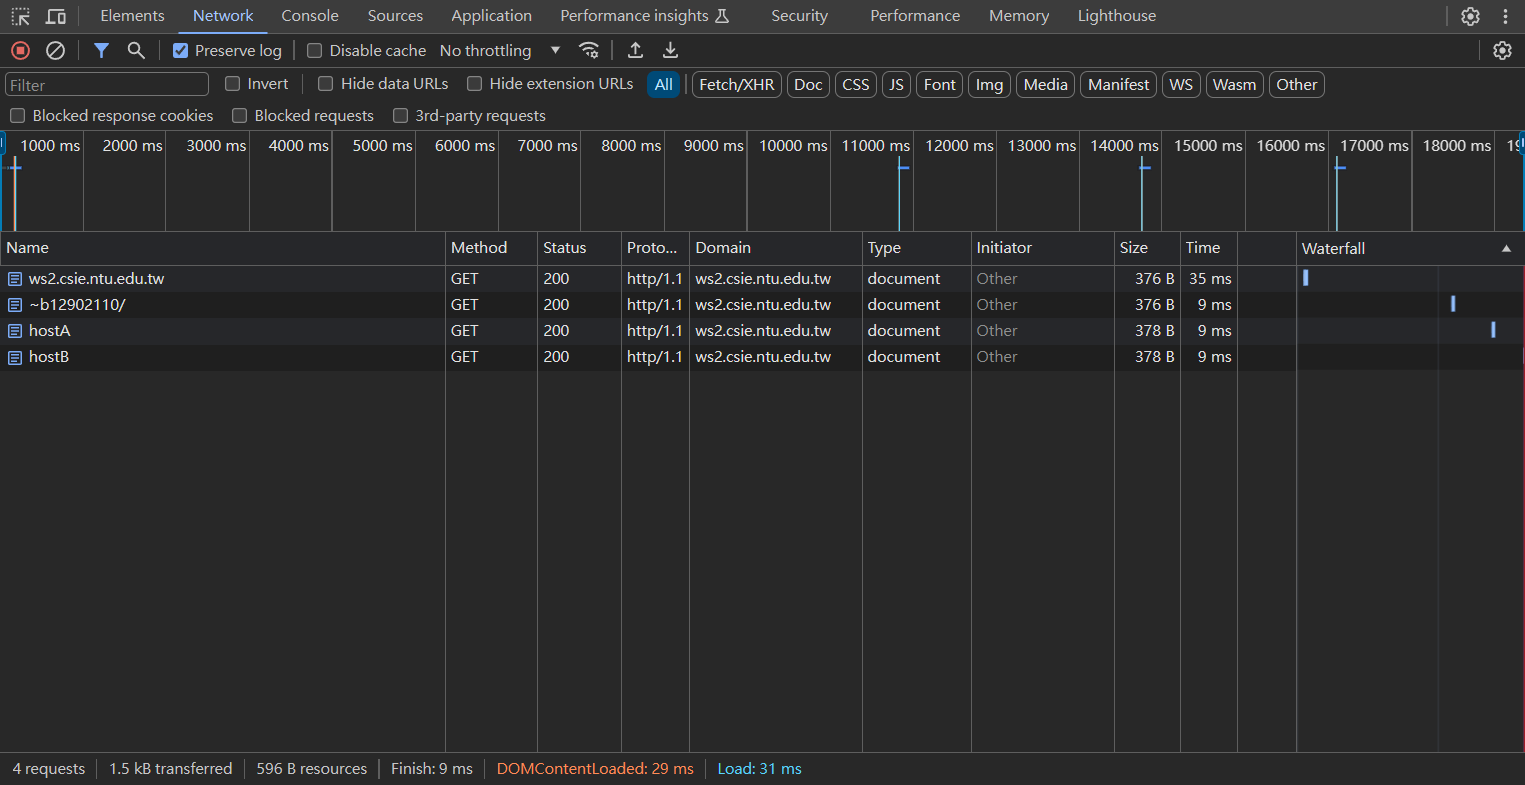
\includegraphics[width=0.93\textwidth]{11_devtools.png}

    \verb|/var/log/nginx/access.log|:

    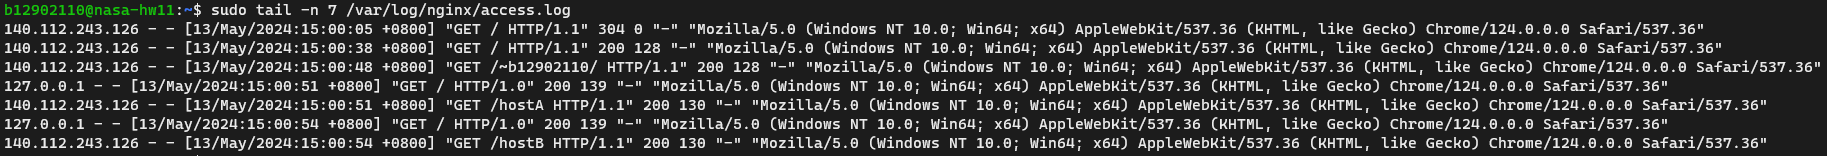
\includegraphics[width=0.93\textwidth]{11_log.png}

    \vspace{\baselineskip}
    \textbf{References}
    \begin{itemize}
      \item \href{https://docs.nginx.com/nginx/admin-guide/monitoring/logging/}{Configuring Logging | NGINX Documentation}
    \end{itemize}

    \pagebreak
    \item
    \begin{enumerate}
      \item TLS uses PKI in the handshake process to authenticate identities of the
      communicating hosts.

      \item A CA is a trusted third party that issues and signs digital certificates.
    \end{enumerate}

    \textbf{References}
    \begin{itemize}
      \item \href{https://en.wikipedia.org/wiki/Transport_Layer_Security}{Transport Layer Security - Wikipedia}
      \item \href{https://en.wikipedia.org/wiki/Public_key_infrastructure}{Public key infrastructure - Wikipedia}
    \end{itemize}

    \begin{enumerate}[resume]
      \item \textbf{Steps (Server)}
      \begin{enumerate}[label=(\arabic*)]
        \item Create an CA key and certificate.
        \begin{Verbatim}[frame=single]
$ openssl req -new -x509 -noenc -days 365000 -newkey rsa:2048 \
    -keyout ca-key.pem -out ca-cert.pem \
    -subj "/C=TW/O=NTU CSIE/OU=NASA/CN=b12902110 Root CA"
        \end{Verbatim}
        \item Create a server key and certificate request.
        \begin{Verbatim}[frame=single]
$ openssl req -new -noenc -newkey rsa:2048 \
    -keyout server-key.pem -out server-req.pem \
    -subj "/C=TW/O=NTU CSIE/OU=NASA/CN=nasa-hw11" \
    -addext "subjectAltName = DNS:*.csie.ntu.edu.tw"
        \end{Verbatim}
        \item Sign the server certificate.
        \begin{Verbatim}[frame=single]
$ openssl x509 -req -days 365000 -copy_extensions copyall \
    -in server-req.pem -out server-cert.pem \
    -CA ca-cert.pem -CAkey ca-key.pem
Certificate request self-signature ok
subject=C = TW, O = NTU CSIE, OU = NASA, CN = nasa-hw11
        \end{Verbatim}

        \item Install the certificate and key to \verb|/etc/nginx|.
        \begin{Verbatim}[frame=single]
$ sudo cp server-key.pem server-cert.pem /etc/nginx
$ sudo chown www-data:www-data /etc/nginx/server-key.pem
        \end{Verbatim}
        \item Add the following directives in \verb|/etc/nginx/sites-available/default|.
        \begin{Verbatim}[frame=single]
server {
  ...

  listen 443 ssl default_server;
  listen [::]:443 ssl default_server;
  ssl_certificate server-cert.pem;
  ssl_certificate_key server-key.pem;

  ...
}
        \end{Verbatim}
        \item Reload the nginx service.
        \begin{Verbatim}[frame=single]
$ sudo systemctl reload nginx.service
        \end{Verbatim}
      \end{enumerate}

      \pagebreak
      \textbf{Steps (Windows Client)}

      Run \verb|certmgr.msc|, and install \verb|ca-cert.pem| to
      ``Trusted Root Certification Authorities".

      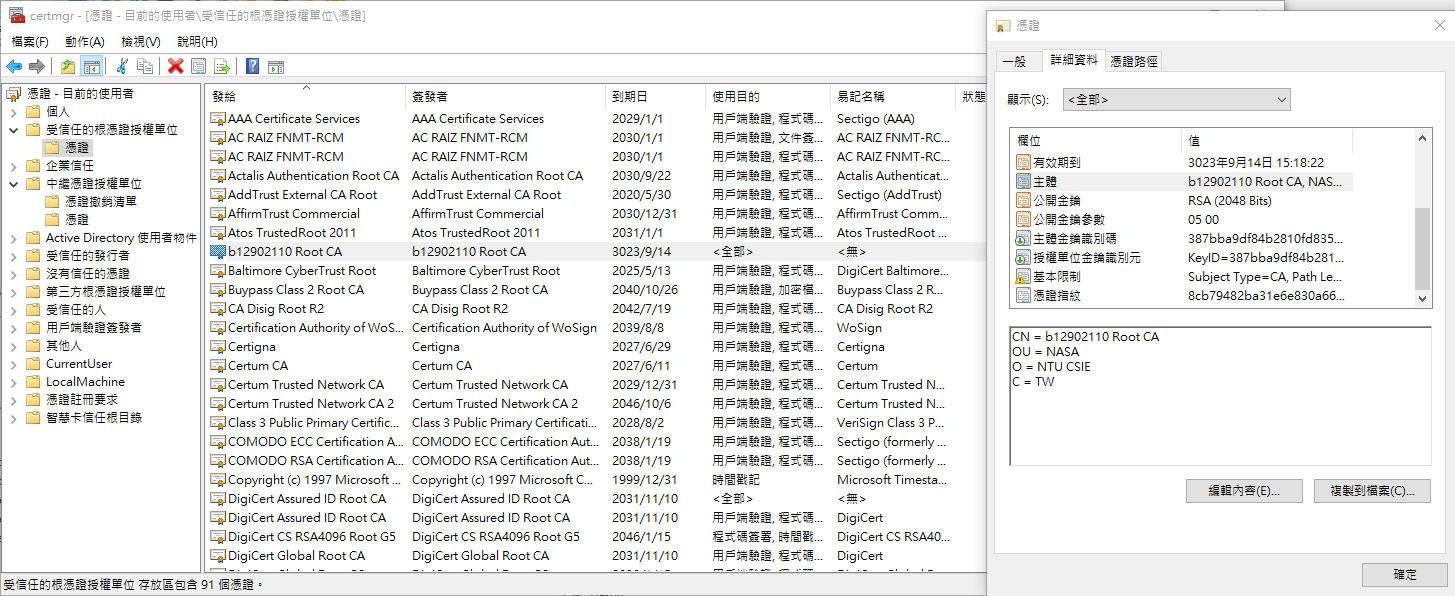
\includegraphics[width=0.87\textwidth]{12-c_certmgr.png}

      \vspace{\baselineskip}
      \textbf{Result}

      Certificates:

      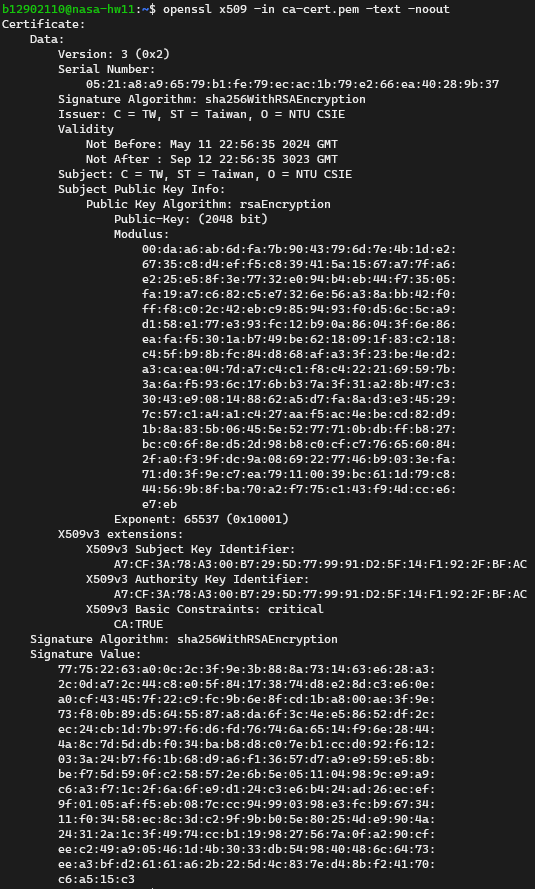
\includegraphics[width=0.43\textwidth]{12-c_ca-cert.png}
      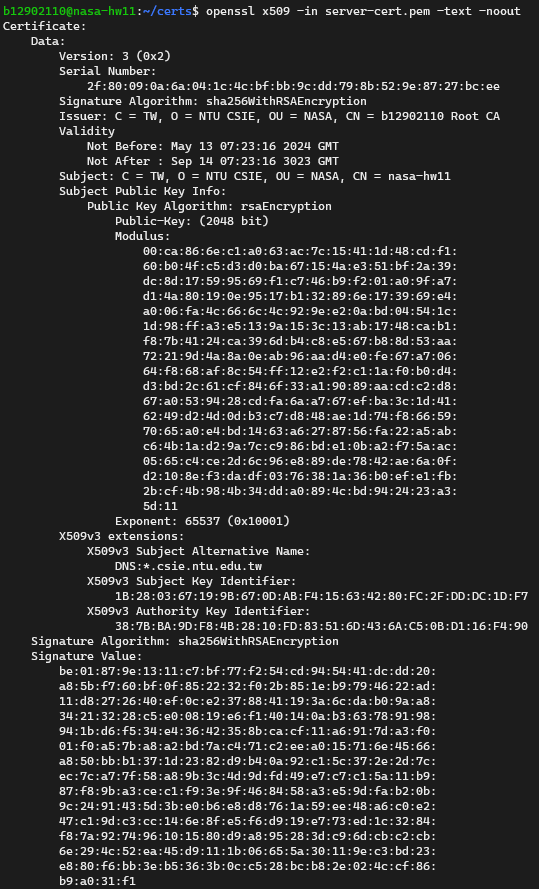
\includegraphics[width=0.43\textwidth]{12-c_server-cert.png}

      \pagebreak
      Browser:

      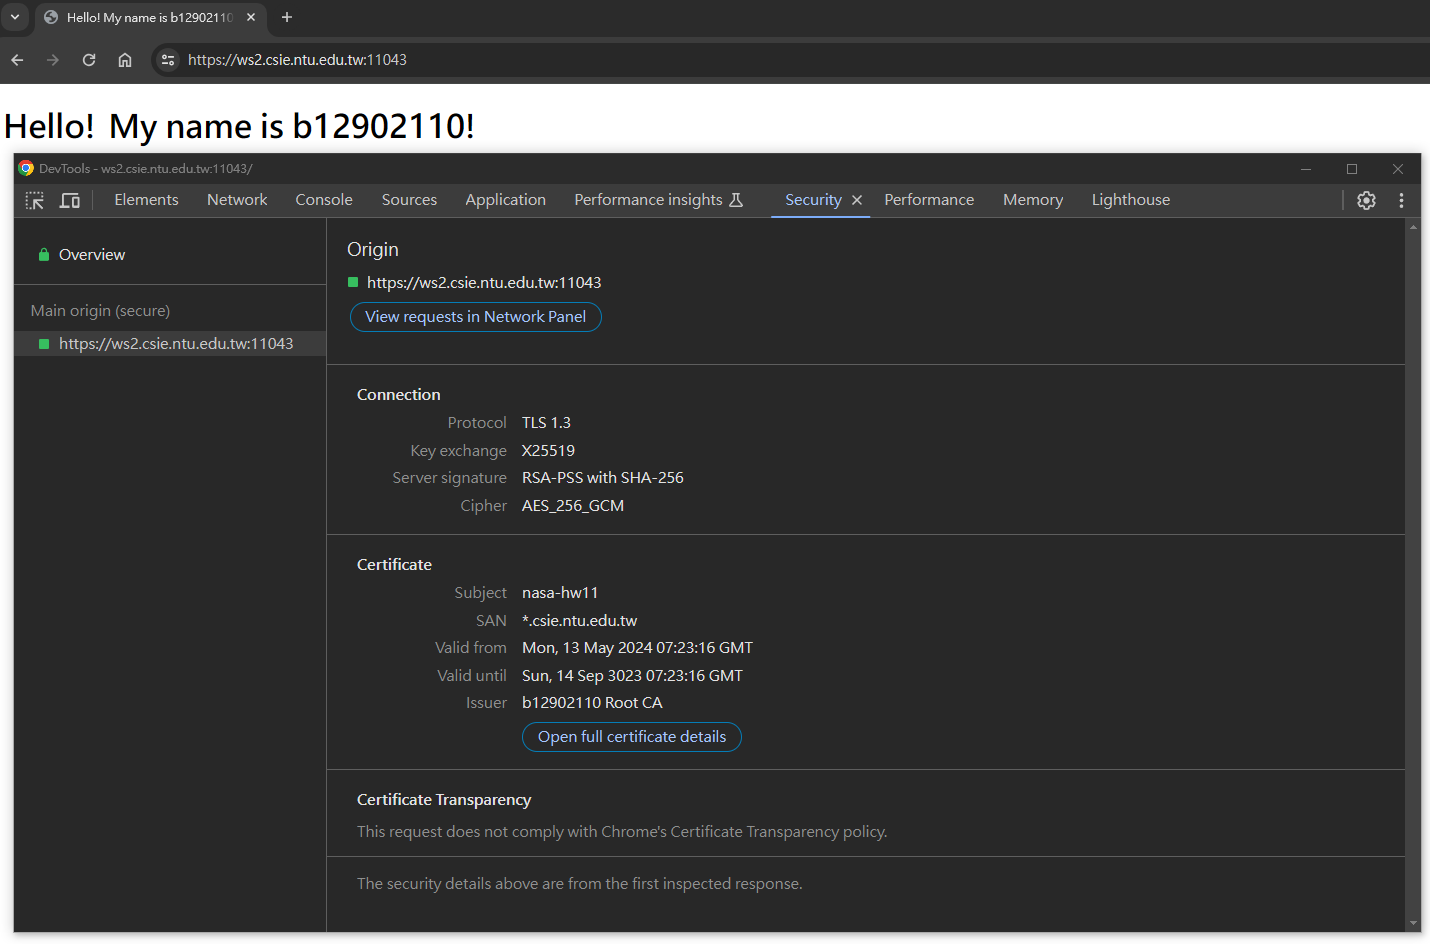
\includegraphics[width=0.87\textwidth]{12-c_browser.png}

      \vspace{\baselineskip}
      \textbf{References}
      \begin{itemize}
        \item \href{https://mariadb.com/docs/server/security/data-in-transit-encryption/create-self-signed-certificates-keys-openssl/}{Create Self-Signed Certificates and Keys with OpenSSL — MariaDB Documentation}
        \item \href{https://www.openssl.org/docs/man3.0/man1/openssl-req.html}{/docs/man3.0/man1/openssl-req.html}
        \item \href{https://www.openssl.org/docs/man3.0/man1/openssl-x509.html}{/docs/man3.0/man1/openssl-x509.html}
        \item \href{https://security.stackexchange.com/questions/74345/provide-subjectaltname-to-openssl-directly-on-the-command-line}{certificates - Provide subjectAltName to openssl directly on the command line - Information Security Stack Exchange}
      \end{itemize}
    \end{enumerate}
  \end{enumerate}

  \pagebreak
  \section*{Reverse Proxy}
  \begin{enumerate}[resume]
    \item \textbf{Steps}
    \begin{enumerate}[label=(\arabic*)]
      \item Create \verb|/etc/nginx/sites-available/hostA| as the following.
      \inputminted{nginx}{server/etc/nginx/sites-available/hostA}
      \item Create \verb|/etc/nginx/sites-available/hostB| as the following.
      \inputminted{nginx}{server/etc/nginx/sites-available/hostB}
      \item Enable both \verb|hostA| and \verb|hostB|.
      \begin{Verbatim}[frame=single]
$ sudo ln -s /etc/nginx/sites-available/hostA \
    /etc/nginx/sites-enabled/hostA
$ sudo ln -s /etc/nginx/sites-available/hostB \
    /etc/nginx/sites-enabled/hostB
      \end{Verbatim}
      \item Create \verb|/var/www/hostA/index.html| as the following.
      \inputminted{html}{server/var/www/hostA/index.html}
      \item Create \verb|/var/www/hostB/index.html| as the following.
      \inputminted{html}{server/var/www/hostB/index.html}
      \item Add \verb|/hostA| and \verb|/hostB| location blocks to
      \verb|/etc/nginx/sites-available/default|.
      \begin{Verbatim}[frame=single]
server {
  ...

  location /hostA {
    proxy_pass http://127.0.0.1:8888/;
  }

  location /hostB {
    proxy_pass http://127.0.0.1:9999/;
  }

  ...
}
      \end{Verbatim}
      \item Reload the nginx service.
      \begin{Verbatim}[frame=single]
$ sudo systemctl reload nginx.service
      \end{Verbatim}
    \end{enumerate}

    \textbf{Result}

    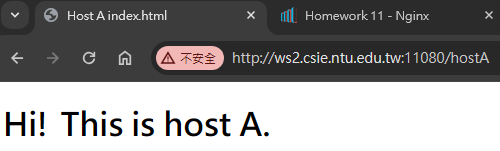
\includegraphics[width=0.45\textwidth]{13_hostA.png}
    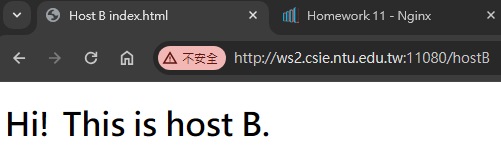
\includegraphics[width=0.45\textwidth]{13_hostB.png}

    \vspace{\baselineskip}
    \textbf{References}
    \begin{itemize}
      \item \href{https://nginx.org/en/docs/beginners_guide.html}{Beginner's Guide}
      \item \href{https://nginx.org/en/docs/http/ngx_http_proxy_module.html}{Module ngx\_http\_proxy\_module}
    \end{itemize}
  \end{enumerate}
\end{document}
